\documentclass[sigconf,10pt]{acmart}

\usepackage[english]{babel}
\usepackage{blindtext}
\usepackage[ruled,vlined]{algorithm2e} % Abhik: For writing queuing algorithm
% \hypersetup{draft} % Abhik: Debug only. Should NOT be enabled
\usepackage{subfig}
\usepackage{multirow}
%%%%% To handle overflow of long URL references
\usepackage{url}
\usepackage[normalem]{ulem} % For strikethrough
\def\UrlBreaks{\do\/\do-}
%%%%%%%

\newcommand\blfootnote[1]{%
  \begingroup
  \renewcommand\thefootnote{}\footnote{#1}%
  \addtocounter{footnote}{-1}%
  \endgroup
}

% Copyright
% \renewcommand\footnotetextcopyrightpermission[1]{} % removes footnote with conference info
% \setcopyright{none}

%% Rights management information.  This information is sent to you
%% when you complete the rights form.  These commands have SAMPLE
%% values in them; it is your responsibility as an author to replace
%% the commands and values with those provided to you when you
%% complete the rights form.
\acmYear{2021}\copyrightyear{2021}
\setcopyright{acmcopyright}
\acmConference[APNet 2021]{5th Asia-Pacific Workshop on Networking (APNet 2021)}{June 24--25, 2021}{Shenzhen, China}
\acmBooktitle{5th Asia-Pacific Workshop on Networking (APNet 2021) (APNet 2021), June 24--25, 2021, Shenzhen, China}
\acmPrice{15.00}
\acmDOI{10.1145/3469393.3469400}
\acmISBN{978-1-4503-8587-9/21/06}
%\setcopyright{acmcopyright}
%\setcopyright{acmlicensed}
%\setcopyright{rightsretained}
%\setcopyright{usgov}
%\setcopyright{usgovmixed}
%\setcopyright{cagov}
%\setcopyright{cagovmixed}

\settopmatter{printacmref=true, printccs=true, printfolios=true}

% DOI
% \acmDOI{}

% ISBN
% \acmISBN{}

%Conference
%\acmConference[Submitted for review to SIGCOMM]{}
%\acmYear{2018}
%\copyrightyear{}

%% {} with no args suppresses printing of the price
% \acmPrice{}


\begin{document}
\title[Leveraging Programmable Dataplanes for a High Performance 5G UPF]{Leveraging Programmable Dataplanes for a High Performance 5G User Plane Function}

%\titlenote{Produces the permission block, and copyright information}
%\subtitle{Extended Abstract}

% \author{Paper \# XXX, XXX pages}
\author{Abhik Bose\footnotemark[1], Diptyaroop Maji\footnotemark[1], Prateek Agarwal, Nilesh Unhale, Rinku Shah, Mythili Vutukuru}
% \thanks{Student authors with equal contribution.}
% \footnotemark[1]
\affiliation{%
  \institution{Department of Computer Science \& Engineering\\
  Indian Institute of Technology Bombay}
}
\email{{abhik, diptyaroop, prateekag, nileshunhale, rinku, mythili}@cse.iitb.ac.in}

% \author{Abhik Bose, Diptyaroop Maji} 
% \author{Prateek Agarwal, Nilesh Unhale, Rinku Shah, Mythili Vutukuru}
% % \thanks{Student authors with equal contribution.}
% % \footnotemark[1]
% \affiliation{%
%   \institution{Department of Computer Science \& Engineering\\
%   Indian Institute of Technology Bombay}
% }
% \email{{abhik, diptyaroop, prateekag, nileshunhale, rinku, mythili}@cse.iitb.ac.in}
% 

% The default list of authors is too long for headers}
\renewcommand{\shortauthors}{Abhik Bose, et al.}
% \author{Firstname Lastname}
% \authornote{Note}
% \orcid{1234-5678-9012}
% \affiliation{%
%   \institution{Affiliation}
%   \streetaddress{Address}
%   \city{City} 
%   \state{State} 
%   \postcode{Zipcode}
% }
% \email{email@domain.com}

% The default list of authors is too long for headers}
% \renewcommand{\shortauthors}{X.et al.}

\begin{abstract}
   % \blindtext
   %Recent technological advancements have encouraged several diverse application domains to provide mobile services. 
Emerging 5G applications require a dataplane that has a high forwarding throughput and low processing latency, in addition to low cost and power consumption. 
%Certain mobile services require ultra-low end-to-end user plane latencies, ranging from {\em{10ms}} to {\em{50ms}}, which the state-of-the-art UPF solutions do not support. 
To meet these requirements, the state-of-the-art 5G User Plane Functions (UPFs) are built over high performance packet I/O mechanisms like the Data Plane Development Kit (DPDK), and further offload some functionality to programmable dataplane hardware. In this paper, we design and implement several standards-compliant UPF prototypes, beginning with a software-only DPDK-based UPF, progressing to designs which offload different functions to programmable hardware. We evaluate and compare the performance of these designs, to highlight the costs and benefits of these offloads. Our results show that offload techniques employed in prior work help improve performance in certain scenarios, but also have their limitations. Overcoming these limitations and fully realizing the power of programmable hardware requires offloading more complex functionality than is done today. Our work presents a preliminary implementation towards a comprehensive programmable dataplane-accelerated 5G UPF. 

%In this paper, we identify the UPF functionalities that can be accelerated using the programmable network hardware. We discuss various offload choices along with the advantages and limitations of each option. We also identify the challenges in the offload and discuss the possible solutions. Our initial prototype evaluation demonstrated up to XXX\% reduction in end-to-end latency, and we estimate up to XXX\%  of power savings.
\end{abstract}

\begin{CCSXML}
<ccs2012>
   <concept>
       <concept_id>10003033.10003099.10003103</concept_id>
       <concept_desc>Networks~In-network processing</concept_desc>
       <concept_significance>500</concept_significance>
       </concept>
   <concept>
       <concept_id>10003033.10003099.10003102</concept_id>
       <concept_desc>Networks~Programmable networks</concept_desc>
       <concept_significance>500</concept_significance>
       </concept>
   <concept>
       <concept_id>10003033.10003079.10011672</concept_id>
       <concept_desc>Networks~Network performance analysis</concept_desc>
       <concept_significance>300</concept_significance>
       </concept>
   <concept>
       <concept_id>10003033.10003106.10003113</concept_id>
       <concept_desc>Networks~Mobile networks</concept_desc>
       <concept_significance>500</concept_significance>
       </concept>
 </ccs2012>
\end{CCSXML}

\ccsdesc[500]{Networks~In-network processing}
\ccsdesc[500]{Networks~Programmable networks}
\ccsdesc[300]{Networks~Network performance analysis}
\ccsdesc[500]{Networks~Mobile networks}

%%
%% Keywords. The author(s) should pick words that accurately describe
%% the work being presented. Separate the keywords with commas.
\keywords{5G core, cellular networks, programmable networks, DPDK, in-network compute}

\maketitle
\vspace{-8pt}
\section{Introduction} \label{sec:intro}
\blfootnote{\textsuperscript{\normalsize*} Student authors with equal contribution.}
% State-of-the-art 5G designs
% Challenges
% Motivation
% Problem statement
% Contribution
% \vspace{-2pt}
The growth in mobile services and subscribers has resulted in an exponential increase in mobile signaling and data traffic~\cite{stats-ericsson, stats-1, stats-2, 5g-stats}. The upcoming 5G standards aim to support applications with diverse traffic characteristics and requirements like enhanced mobile broadband, dense deployments of IoT devices, self-driving cars, and AR/VR~\cite{ngmn, 5g-iot-chk}. These applications require high throughput, very low processing latencies, and stringent Quality-of-Service (QoS) enforcement. The mobile packet core, which connects the radio access network to external networks, comprises of control plane components that process signaling messages and a dataplane that forwards user traffic. The User Plane Function (UPF) is the main entity in the dataplane of the future 5G mobile packet core, and has a significant impact on the performance that users are going to perceive with 5G. 

\begin{table}[t]
\begin{scriptsize}
\begin{center}
\def\arraystretch{1.5}%  1 is the default, change whatever you need
\begin{tabular}{|p{1.7cm}|p{0.9cm}|p{0.7cm}|p{0.7cm}|p{0.7cm}|p{1.4cm}|}\hline 
% {\bf{}} & {\bf{Server}} & {\bf{Agilio CX 2x10GbE}} & {\bf{Agilio CX 2x25GbE}} & {\bf{Agilio CX 2x40GbE}} & {\bf{Tofino switch ASIC}}  \\ 
&  \multirow{2}{*}{\bf{Server}} & \multicolumn{3}{c|}{\bf{Agilio CX SmartNICs~\cite{netronome-cx-4000,netronome-cost}}} & \multirow{2}{*}{\bf{Tofino switch}}  \\ %\hline
& {\bf{\cite{xeon-processor, 40G-nic-cost}}}  &  {\bf{\cite{netronome}}} &  {\bf{\cite{netronome-25G}}}   & {\bf{\cite{netronome-40G}}}  & {\bf{\cite{tofino-2}}}  \\ \hline 
% & & {\textbf{10GbE}} & {\textbf{25GbE}} & {\textbf{40GbE}} & \\ \hline
 
% {\bf{Mbps per USD}} & 50  & 23  & 47 & 65 & 544 \\ \hline
% {\bf{Mbps per Watt}} & 222  & 200 & 500 & 800 & 11480 \\ \hline
{\bf{Mpps per USD}} & 0.03 & 0.33  & 0.28 & 0.24  & 0.4  \\ \hline
{\bf{Mpps per Watt}} & 0.14 & 2.96 & 2.96 & 2.96 & 8.52  \\ \hline
\end{tabular}
\setlength{\abovecaptionskip}{-12pt}
\setlength{\belowcaptionskip}{0pt}
\caption{Performance per unit cost and power.} 
\label{tab:cost-power}
\end{center}
\end{scriptsize}
\end{table}

% \begin{table}[t]
% \begin{scriptsize}
% \begin{center}
% \def\arraystretch{1.5}%  1 is the default, change whatever you need
% \begin{tabular}{|p{1.7cm}|p{0.9cm}|p{1cm}|p{1cm}|p{0.9cm}|p{0.8cm}|}\hline 
% {\bf{}} & {\bf{Intel Xeon CPU}} & {\bf{Agilio CX 2x10GbE}} & {\bf{Agilio CX 2x25GbE}} & {\bf{Agilio CX 2x40GbE}} & {\bf{Tofino switch ASIC}}  \\ 
% 
% {\bf{}} & {\bf{\cite{xeon-processor, 40G-nic-cost}}}  &  {\bf{\cite{netronome-cx-4000, netronome-cost}}} & {\bf{\cite{netronome-cx-4000, netronome-cost}}} & {\bf{\cite{netronome-cx-4000, netronome-cost}}} & {\bf{\cite{tofino-2}}}  \\ \hline 
% 
% % {\bf{Mbps per USD}} & 50  & 23  & 47 & 65 & 544 \\ \hline
% % {\bf{Mbps per Watt}} & 222  & 200 & 500 & 800 & 11480 \\ \hline
% {\bf{Mpps per USD}} & 0.03 & 0.33  & 0.28 & 0.24  & 0.4  \\ \hline
% {\bf{Mpps per Watt}} & 0.14 & 2.96 & 2.96 & 2.96 & 8.52  \\ \hline
% \end{tabular}
% \setlength{\abovecaptionskip}{-12pt}
% % \setlength{\belowcaptionskip}{-8pt}
% \caption{Performance per unit cost and power.} 
% \label{tab:cost-power}
% \end{center}
% \end{scriptsize}
% \end{table}

Most state-of-the-art UPFs are built as multicore-scalable software packet processing appliances running over commodity servers, and process traffic using a high performance packet I/O mechanism like the Data Plane Development Kit (DPDK)~\cite{dpdk_overview}. However, given the stringent performance requirements of 5G networks~\cite{ngmn, 5g-iot-chk}, and ever increasing network speeds running into hundreds of Gbps, offloading some UPF packet processing to programmable dataplane hardware can lead to improved performance, along with cost and power savings. We establish this benefit of offload in Table~\ref{tab:cost-power}, which shows the data forwarding capacity per unit cost/power for various programmable hardware platforms as well as a general purpose server CPU core that all run a UPF. We obtain this table as follows: the UPF throughput values for the first two columns (single core server and Agilio CX 2x10GbE) were measured using our standards-compliant UPF implementations (\S\ref{sec:design}), while we assumed that the other hardware platforms were capable of handling offloaded UPF processing at linerate (a reasonable assumption from our experience with one platform). The cost and power consumption were obtained from the hardware specifications. We see from the table that offloading UPF processing to programmable hardware can result in significant cost and power savings across a wide variety of programmable dataplane platforms. The idea of accelerating UPF using programmable hardware is not new---prior work  has proposed offloading the logic of steering packets to multiple CPU cores of the UPF~\cite{astri, intel_wp, mavenir, metaswitch}, as well as the dataplane forwarding itself~\cite{astri, mobile_5G_hw1, mobile_5G_hw2, mavenir, kaloom_wp}. However, to the best of our knowledge, none of the existing works systematically enumerates all the possible ways in which UPF functionality can be offloaded to programmable hardware, nor do they precisely quantify the costs and benefits of such offloads. 

%there has been significant interest from both industry and academia in exploring the recent technological advances of programmable dataplane hardware to accelerate pure software-based UPFs~\cite{astri, mobile_5G_hw1, mobile_5G_hw2, mavenir, intel_wp, kaloom_wp, turboEPC, metaswitch}. The purported benefits of such an offload are widely accepted---hardware platforms can more easily perform complex processing at linerate, leading to lower cost, lower power consumption, and better processing latencies. 

In this work, we begin with an industry-grade software based UPF built over DPDK, and progressively offload functions to programmable hardware, to come up with several different UPF prototypes (\S\ref{sec:design}). We then measure the throughput and latency characteristics of such UPFs to analyze the pros and cons of offloading UPF functionality to programmable hardware (\S\ref{sec:eval}). For example, we find that offloading the logic of steering packets to the multiple CPU cores reduces UPF processing latency by up to $37 \%$ and increases throughput by $45 \%$. However, performing packet steering in hardware is less flexible than doing so in software, and performs badly during scenarios involving dynamic scaling and skewed traffic distribution across users. Another interesting observation is that, while forwarding data directly from the programmable dataplane hardware (rather than via userspace) leads up to $24$\% lower latency in the dataplane as expected, it significantly worsens the control plane performance. This is because the UPF continues to process signaling messages (from the control plane that configures forwarding rules) within userspace itself, and in this split architecture, the communication between the UPF software and the programmable hardware becomes the bottleneck.\texttt{}
% XXX: SteerOffload decreases latency by 40\% while PartialOffload decreases latency by 5-30\%. Will the create confusion? Should we mention about different setups upfront?

In this paper, we posit that truly leveraging the performance of programmable hardware to accelerate the 5G dataplane requires the UPF to process and respond to signaling messages from the hardware itself, in order not be limited by the hardware configuring capacity of userspace software. This is challenging to do for several reasons, including the variable-sized message formats of UPF signaling messages. This paper provides a preliminary implementation that solves some of these challenges, and provides initial results that show the promise of offloading these complex UPF functions to programmable hardware. Our work paves the way towards a high-performance 5G UPF that fully leverages the power of programmable dataplanes. 


% \begin{table}[ht]
% \begin{scriptsize}
% \begin{center}
% \def\arraystretch{1.5}%  1 is the default, change whatever you need
% \begin{tabular}{|p{1cm}|p{1.2cm}|p{1.2cm}|p{1.2cm}|p{1cm}|p{1cm}|}\hline 
% {\bf{}} & {\bf{10GbE NPU~\cite{netronome-cx-4000}}} & {\bf{25GbE NPU~\cite{netronome-cx-4000}}} & {\bf{40GbE NPU~\cite{netronome-cx-4000}}} & {\bf{Tofino switch ASIC~\cite{tofino-2}}} & {\bf{Intel Xeon CPU~\cite{xeon-processor}}} \\ \hline 
% {\bf{Mbps per USD}} & 22.52  & 47.44 & 65.47 & 544.68  & 2.72 \\ \hline
% {\bf{Mbps per Watt}} & 200 & 500 & 800 & 11480 & 83  \\ \hline
% {\bf{Mpps per USD}} & 0.33  & 0.28 & 0.24  & 0.4 & 0.04  \\ \hline
% {\bf{Mpps per Watt}} & 2.96 & 2.96 & 2.96 & 8.52 & 1.17 \\ \hline
% \end{tabular}
% % \setlength{\abovecaptionskip}{-5pt}
% % \setlength{\belowcaptionskip}{ 8pt}
% \caption{Hardware performance with respect to per unit cost and power. XXX: Needs fixing. Talk to me for comments.} 
% \label{tab:cost-power}
% \end{center}
% \end{scriptsize}
% \end{table}

%Table~\ref{tab:cost-power} {\textbf {(XXX: keep Mbps or Mpps? Put this in intro to motivate hardware offload?)}} shows the performance per unit cost and the performance per unit power for a variety of programmable hardware and the server used in our experiment. We have derived these metrics using the device specifications~\cite{netronome-cx-4000, tofino-2, xeon-processor}.
%We observe that all programmable hardware provide better performance per unit cost/power compared to the traditional commodity servers. Therefore, we should offload the processing to programmable hardware if we can express our computations.


%\begin{table}[ht]
%\begin{scriptsize}
%\begin{center}
%\def\arraystretch{1.5}%  1 is the default, change whatever you need
%\begin{tabular}{|p{1cm}|p{1.2cm}|p{1.2cm}|p{1.2cm}|p{1cm}|p{1cm}|}\hline 
%{\bf{}} & {\bf{10GbE NPU~\cite{netronome-cx-4000}}} & {\bf{25GbE NPU~\cite{netronome-cx-4000}}} & {\bf{40GbE NPU~\cite{netronome-cx-4000}}} & {\bf{Tofino switch ASIC~\cite{tofino-2}}} & {\bf{Intel Xeon CPU~\cite{xeon-processor}}} \\ \hline 
%{\bf{Mbps per USD}} & 22.52  & 47.44 & 65.47 & 544.68  & 2.72 \\ \hline
%{\bf{Mbps per Watt}} & 200 & 500 & 800 & 11480 & 83  \\ \hline
%{\bf{Mpps per USD}} & 0.33  & 0.28 & 0.24  & 0.4 & 0.04  \\ \hline
%{\bf{Mpps per Watt}} & 2.96 & 2.96 & 2.96 & 8.52 & 1.17 \\ \hline
%\end{tabular}
%% \setlength{\abovecaptionskip}{-5pt}
%% \setlength{\belowcaptionskip}{ 8pt}
%\caption{Hardware performance with respect to per unit cost and power.} 
%\label{tab:cost-power}
%\end{center}
%\end{scriptsize}
%\end{table}
%
%Table~\ref{tab:cost-power} {\textbf {(XXX: keep Mbps or Mpps? Put this in intro to motivate hardware offload?)}} shows the performance per unit cost and the performance per unit power for a variety of programmable hardware and the server used in our experiment. We have derived these metrics using the device specifications~\cite{netronome-cx-4000, tofino-2, xeon-processor}.
%We observe that all programmable hardware provide better performance per unit cost/power compared to the traditional commodity servers. Therefore, we should offload the processing to programmable hardware if we can express our computations.
%


\vspace{-5pt}
\section{Background \& Related Work} \label{sec:bg}
%\subsection{5G Architecture} 
%\label{sub:5g_arch}

\begin{figure}[t]
 \centering
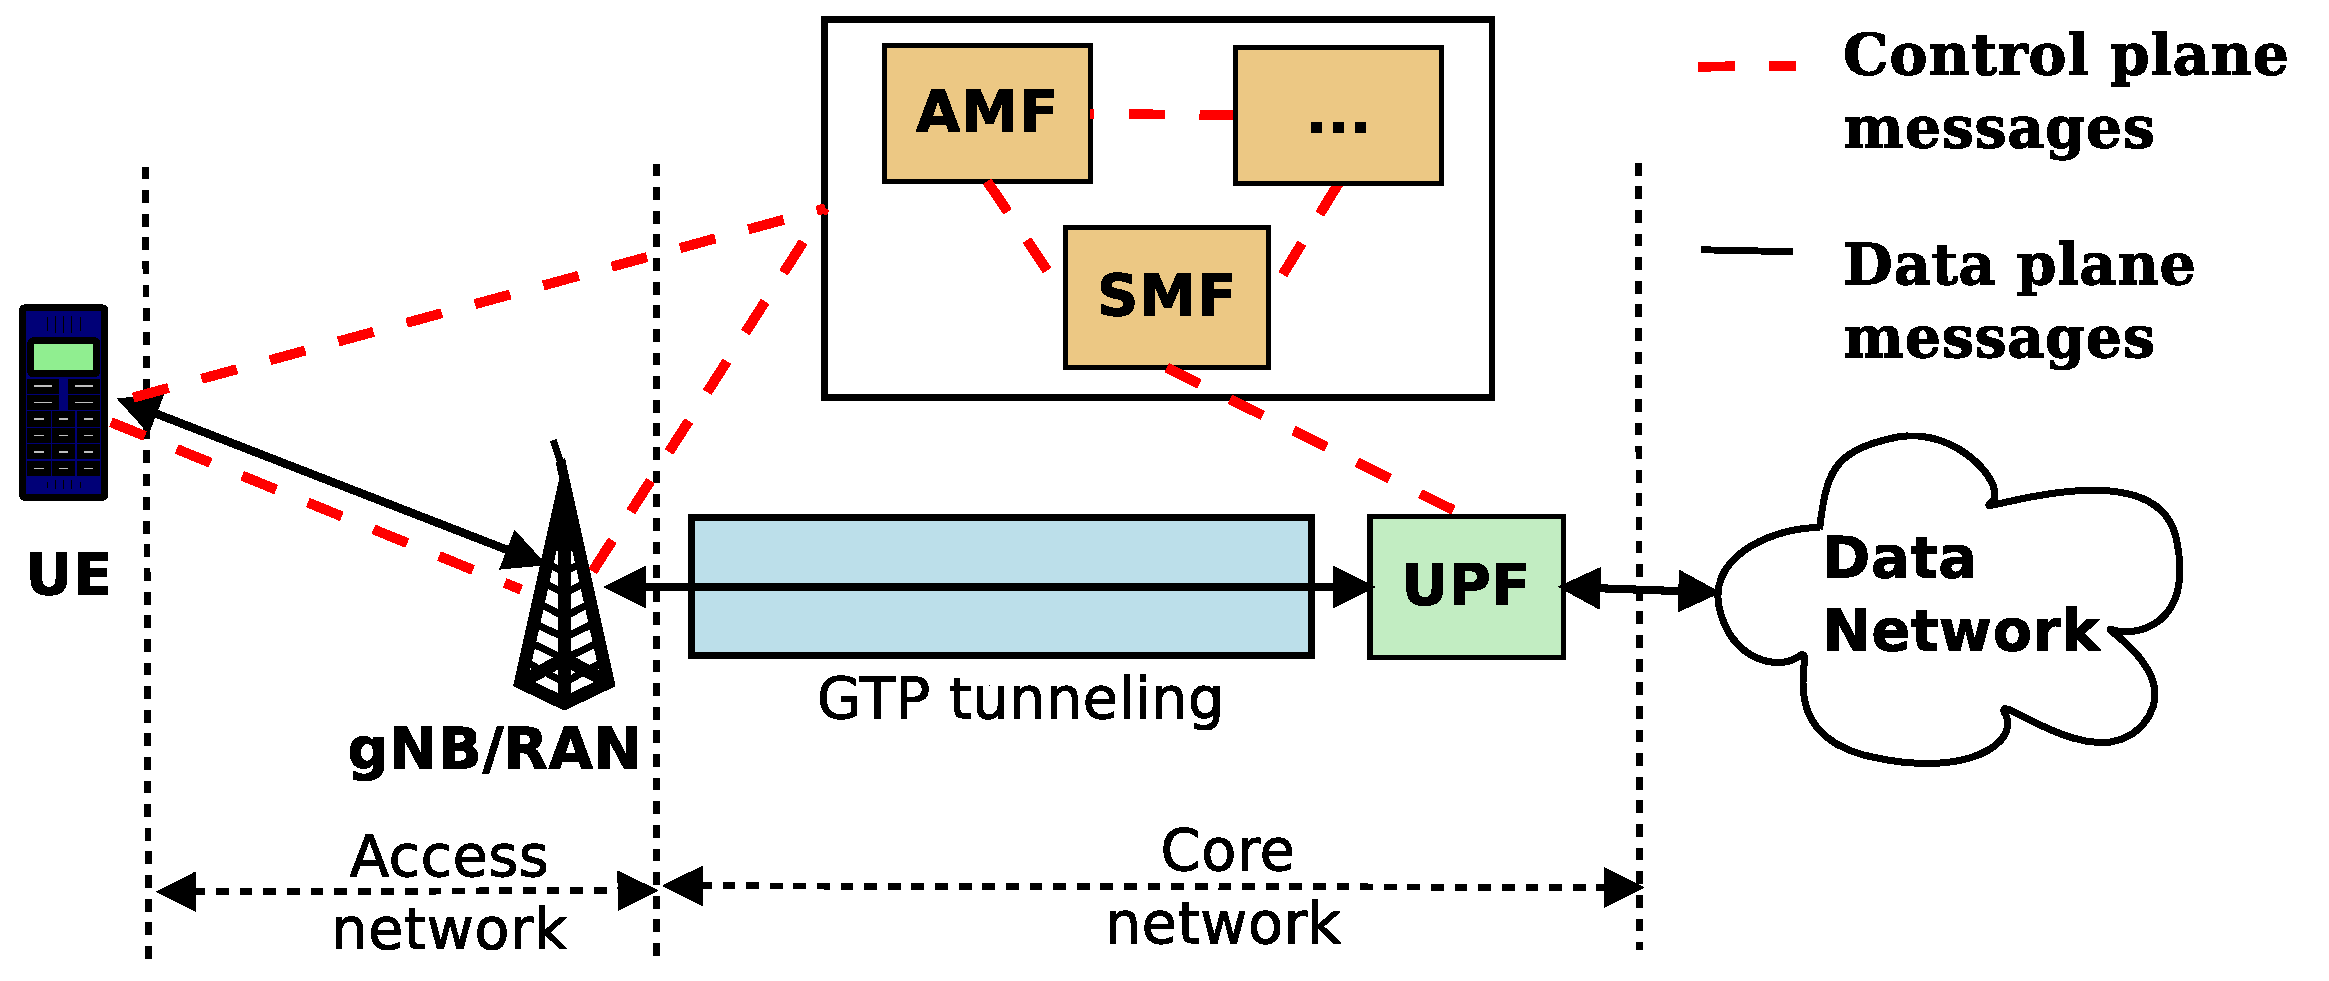
\includegraphics[width=0.4\textwidth]{fig/5g_arch.eps}
%  \setlength{\abovecaptionskip}{-2pt}
\setlength{\belowcaptionskip}{-12pt}
 \caption{5G Architecture.}
 \label{fig:5g_arch}
\end{figure}
%\vspace{-5mm}

\noindent {\bf 5G architecture.} Figure~\ref{fig:5g_arch} shows a high-level overview of the 5G architecture~\cite{5g23501}. A 5G network consists of the wireless radio access network (RAN), which includes the User Equipment (UE) and the Base Station/g-NodeB (gNB), and the wired packet core network. In the control plane of the 5G core, the Access and Mobility Function (AMF) deals with registration and mobility management, and the Session Management Function (SMF) manages the UE's data sessions. The data plane comprises of one or more User Plane Functions (UPFs) that forward user data through the packet core. The control and data plane components communicate using Packet Forwarding Control Protocol (PFCP) messages that are exchanged between the SMF and UPF over UDP~\cite{5g29244}. In the dataplane, a UE's IP datagram packets are encapsulated in GPRS Tunnelling Protocol (GTP) headers when transiting through the packet core; tunnelling aids easy mobility among other things. The GTP-encapsulated IP datagrams are transmitted over a UDP link between the gNB and the UPF. The UPF is responsible for encapsulating downlink packets entering the core with GTP headers and correspondingly decapsulating uplink packets leaving the core. The UPF is also responsible for usage reporting and charging, and enforcing Quality-of-service (QoS), e.g., via rate limiting. 

This paper deals with UPF implementation, so we describe the internal state and data structures at the UPF in more detail. A UE sets up one or more ``sessions'' to forward data through the core, and each data session will cause the SMF to install one or more Packet Detection Rules (PDRs) at the UPF via PFCP messages. A PDR helps associate an incoming data packet to a session based on its GTP/IP packet headers. A PDR has several types of actions associated with it, that instruct the UPF on how to handle the packet. For example, the Forward Action Rules (FARs) specify the forwarding behavior of the packet (e.g., GTP tunnel identifiers for encap), and the QoS Enforcement Rules (QERs) specify the QoS processing to be performed. An example of a field in the QER is the  Aggregate Maximum Bit-Rate (AMBR) of the session. On receiving a PFCP message from the SMF, the UPF creates/updates the required rules, and sends an acknowledgement back to the SMF. On receiving a data packet, the UPF first identifies the matching PDR. For packets belonging to a valid session, the UPF executes forwarding and QoS behavior specified by the FARs and QERs linked to that PDR, in addition to updating usage and charging counters. Packets belonging to ``oversubscribed'' sessions that exceed the rate limit specified in the QoS rules are buffered for an appropriate duration, and scheduled for transmission suitably. 

%%%% Mythili: not sure if we need this figure, can include if there is space.

%Figure~\ref{fig:UPF_DP_proc} shows a simplified data packet processing pipeline in the UPF. 
%
%\begin{figure}[ht]
% \centering
%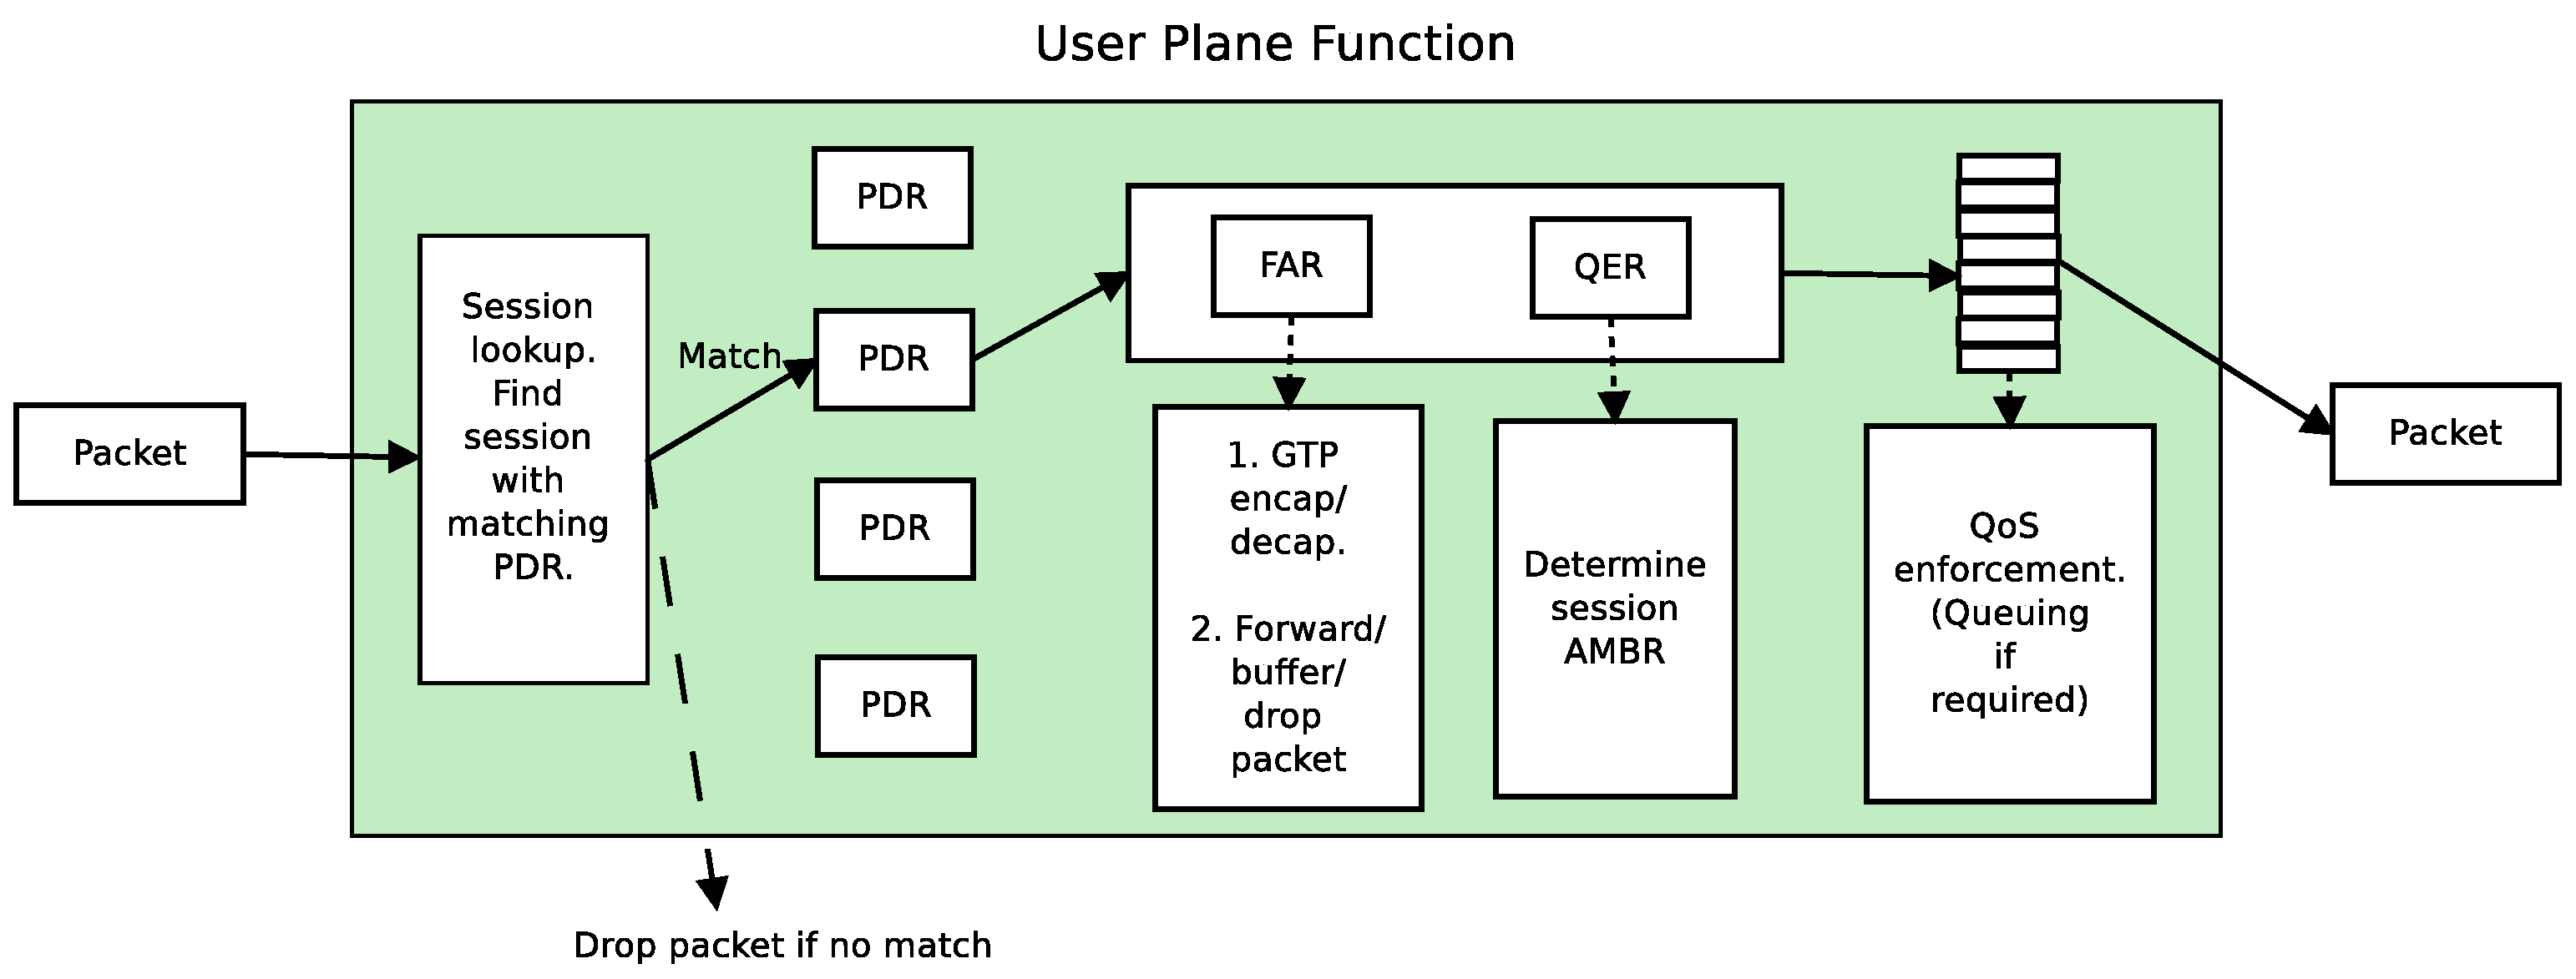
\includegraphics[width=0.5\textwidth]{fig/UPF_DP_processing.eps}
% \setlength{\abovecaptionskip}{6pt}
%% \setlength{\belowcaptionskip}{-6pt}
% \caption{UPF Data Packet processing pipeline.}
% \label{fig:UPF_DP_proc}
%\end{figure}

%%% content below can be deleted after checking once

%
%\noindent \textbf{UPF Data Plane Processing:}
%Fig. \ref{fig:UPF_DP_proc} shows a simplified data packet processing pipeline in the UPF. For each incoming data packet, the UPF browses the existing rules and tries to match the packet against any 1 of the PDRs, based on the packet header fields. If no rule is matched, the UPF discards the packet. If a PDR is matched, it points to the necessary FAR and QER. The UPF may decide whether to forward, buffer or drop the packet, as well as add or remove certain headers based on the FAR. The QER instructs the UPF to enforce necessary QoS. For instance, when a GTP encapsulated data packet for a particular UE arrives at the UPF and a PDR is matched based on the GTP and inner IP header, it will refer to a specific FAR and QER. The FAR may tell the UPF to remove the GTP and outer IP/UDP headers and forward the packet to the DNN. On the other hand, the QER will tell that the UPF should forward packets from that UE at a rate no higher than the specified Aggregate Maximum Bit-Rate (AMBR). To enforce QoS and queue oversubscribed flows in our UPFs, we have implemented the algorithm mentioned in Carousel \cite{carousel} (lines of code: $~XX$) .\\
%% \subsection{P4-SDN-SmartNIC}


%\subsection{State-of-the-art UPFs}

%There are several UPF solutions available today which achieve high performance either by using specialized processing pipelines in s/w or by offloading part of the UPF Data Plane functionalities in the h/w. SK Telecom \cite{intel_wp} uses a SmartNIC to redirect packets to different cores based on Deep Packet Inspection (DPI). 
%% Mavenir \cite{mavenir} compares purely s/w based UPF, UPF with only RSS offloaded, and UPF with both RSS and GTP encapsulation/decapsulation to the h/w in terms of computing costs. 
%Astri \cite{astri} uses Dynamic Device Personalization (DDP) to process packets in the NIC. 
%% Kaloom offloads \cite{kaloom_wp} the Data Plane in h/w. 
%Metaswitch \cite{metaswitch} uses a specilized processing engine (CNAP) in the s/w itself to achive high throughput. However, our work is slightly different from all of the above. We start from a purely s/w based approach and offload the UPF functionalities one by one, comparing the pros ans cons of each design using various metrics. For example, we compare QoS provided, cost per unit of programmable h/w etc. along with regular metrics of throughput and latency in both the Control and the Data Plane. We also propose solutions where queueing in the Data Plane and PFCP parsing in the Control Plane are also offloaded to the h/w.
%
%% \begin{itemize}
%%     \item Intel Whitepaper -- only RSS in h/w
%%     \item Mavenir, APNet-17 -- GTP encap/decap
%%     \item Metaswitch -- P4/gRPC in s/w
%\textbf{[EDIT: Add O-RAN/MEC related work?]}
%% \end{itemize}
 %Diptyaroop
% Add background on 5G architecture, UPF functions and decsription
% related work: Common EPC designs, NF design on DPDK

% \subsection{Offload computations to programmable hardware}
%\vspace{-20pt}

\noindent {\bf Programmable dataplanes.}
Programmable dataplanes allow networking hardware to be easily programmed to perform complex functions, via code written in a high-level language like P4~\cite{p4}. Packet processing pipeline specifications written in P4 can be compiled to a variety of programmable dataplanes, e.g., programmable hardware ASICs \cite{flexpipe, doppler, cavium, tofino}, NPUs \cite{netronome, ezchip}, and FPGAs \cite{xilinx, altera}. The programmable hardware platforms have several limitations put in place, in order to ensure linerate processing. They have limited expressiveness in terms of the supported instruction set and programming constructs, and lack dynamic data-structures. The packets cannot stall during the switch pipeline processing---they have to be either forwarded or dropped. The amount of on-board memory on such hardware is limited ($\sim$few tens of MBs). Despite these limitations, researchers have observed substantial performance benefits by offloading applications to programmable hardware, via creative solutions that address the hardware limitations~\cite{int, hashpipe, network-heavy-hitter, carpe, appswitch, hula, silkroad, netpaxos, in-mem-consensus, netcache, kvdirect, acceltcp, switchml, dream,   blink, wharf}.
%to accelerate software applications, by offloading a part of the application logic to programmable switches or NICs. Some of the popular applications that leverage programmable hardware for performance acceleration include in-band network telemetry~\cite{int}, heavy-hitter flow detection~\cite{hashpipe, network-heavy-hitter, carpe}, stateful load balancers~\cite{appswitch, hula, silkroad}, consensus algorithms~\cite{netpaxos, in-mem-consensus}, key-value caching~\cite{netcache, kvdirect}, TCP processing offload~\cite{acceltcp}, machine learning~\cite{switchml, dream} and network link-failure detection~\cite{blink, wharf}.



%The programmable hardware platforms have several limitations put in place, in order to ensure linerate processing. They have limited expressiveness in terms of the supported instruction set (no multiplication, division, logarithm or polynomial support) and programming constructs (no loops or recursion support), and lack dynamic data-structures. The packets cannot stall during the switch pipeline processing---they have to be either forwarded or dropped. The amount of on-board memory supported on such hardware is limited ($\sim$few tens of MBs). 
%Despite these limitations, researchers have observed substantial performance benefits by offloading their applications to programmable hardware, via creative solutions that address the hardware limitations. 
% 
% \noindent {\textbf{General in-network compute.}}
% The availability of high-level programming language and compilers for the target hardware acts as a catalyst to attract programmers to explore in-network computing. 
%\vspace{-5pt}

\noindent {\bf State-of-the-art UPFs.} Most production grade UPFs are built over kernel-bypass techniques like DPDK to achieve high dataplane throughput in software. Metaswitch \cite{metaswitch} uses a specialized processing engine (CNAP) in the software itself to achieve high throughput. Some UPFs also use programmable hardware or specialized processing engines to offload some part of the UPF processing to hardware. Few proposals~\cite{astri, mobile_5G_hw1, mobile_5G_hw2, mavenir} offload the GTP encap/decap based forwarding to hardware, while some~\cite{intel_wp} offload packet steering to cores via deep packet inspection (DPI) of the inner IP header. Kaloom~\cite{kaloom_wp} offloads a subset of QoS processing (bit rate policing) along with GTP processing to the programmable hardware. Our work explores more offload based designs than those considered in prior work, and systematically analyzes the costs and benefits of the offloads. TurboEPC~\cite{turboEPC} offloads the subset of 4G core signaling messages to the programmable hardware, while our work explores the signaling message offload problem in the context of 5G which has a different architecture. 

%\noindent The telecom community, academia and industry, are working towards designing systems that benefit from in-network compute for the 5G mobile packet core and its applications. 
%
%% SK Telecom \cite{intel_wp} uses a SmartNIC to redirect packets to different cores based on Deep Packet Inspection (DPI). 
%Kaloom~\cite{kaloom_wp} offloads the subset of QoS processing (bit rate policing) along with GTP processing to the programmable hardware. 
%TurboEPC~\cite{turboEPC} offloads the subset of 4G LTE-EPC signaling messages to the programmable hardware. 
%Our goal is to offload the standard compliant 5G UPF dataplane and signaling procedures to provide an accelerated, low cost, and a low power solution.

% % \noindent  {\textbf{In-network compute for telecom applications.}}
% EDIT HERE: 5G RAN acceleration\\
% 4G/5G offload examples: RSS, GTP, control-plane (TurboEPC)\\
% Few proposals~\cite{mobile_5G_hw1, mobile_5G_hw2} offload the GTP header encapsulation and decapsulation processing to the data plane edge switch of the mobile packet core. \\
% 
% Our goal is to offload the data plane as well as the control plane procedures of the 5G UPF and provide an accelerated, low cost, low power solution.





 %Rinku
% General hardware offload literature/P4
% Offload of 4G, 5G (general) : academia + industry (recent work on RAN offload)
% Offloading of UPF: Industry white papers
% General in-network compute

\vspace{-5mm}
\section{Design \& Implementation} \label{sec:design}
\begin{figure}[t]
 \centering
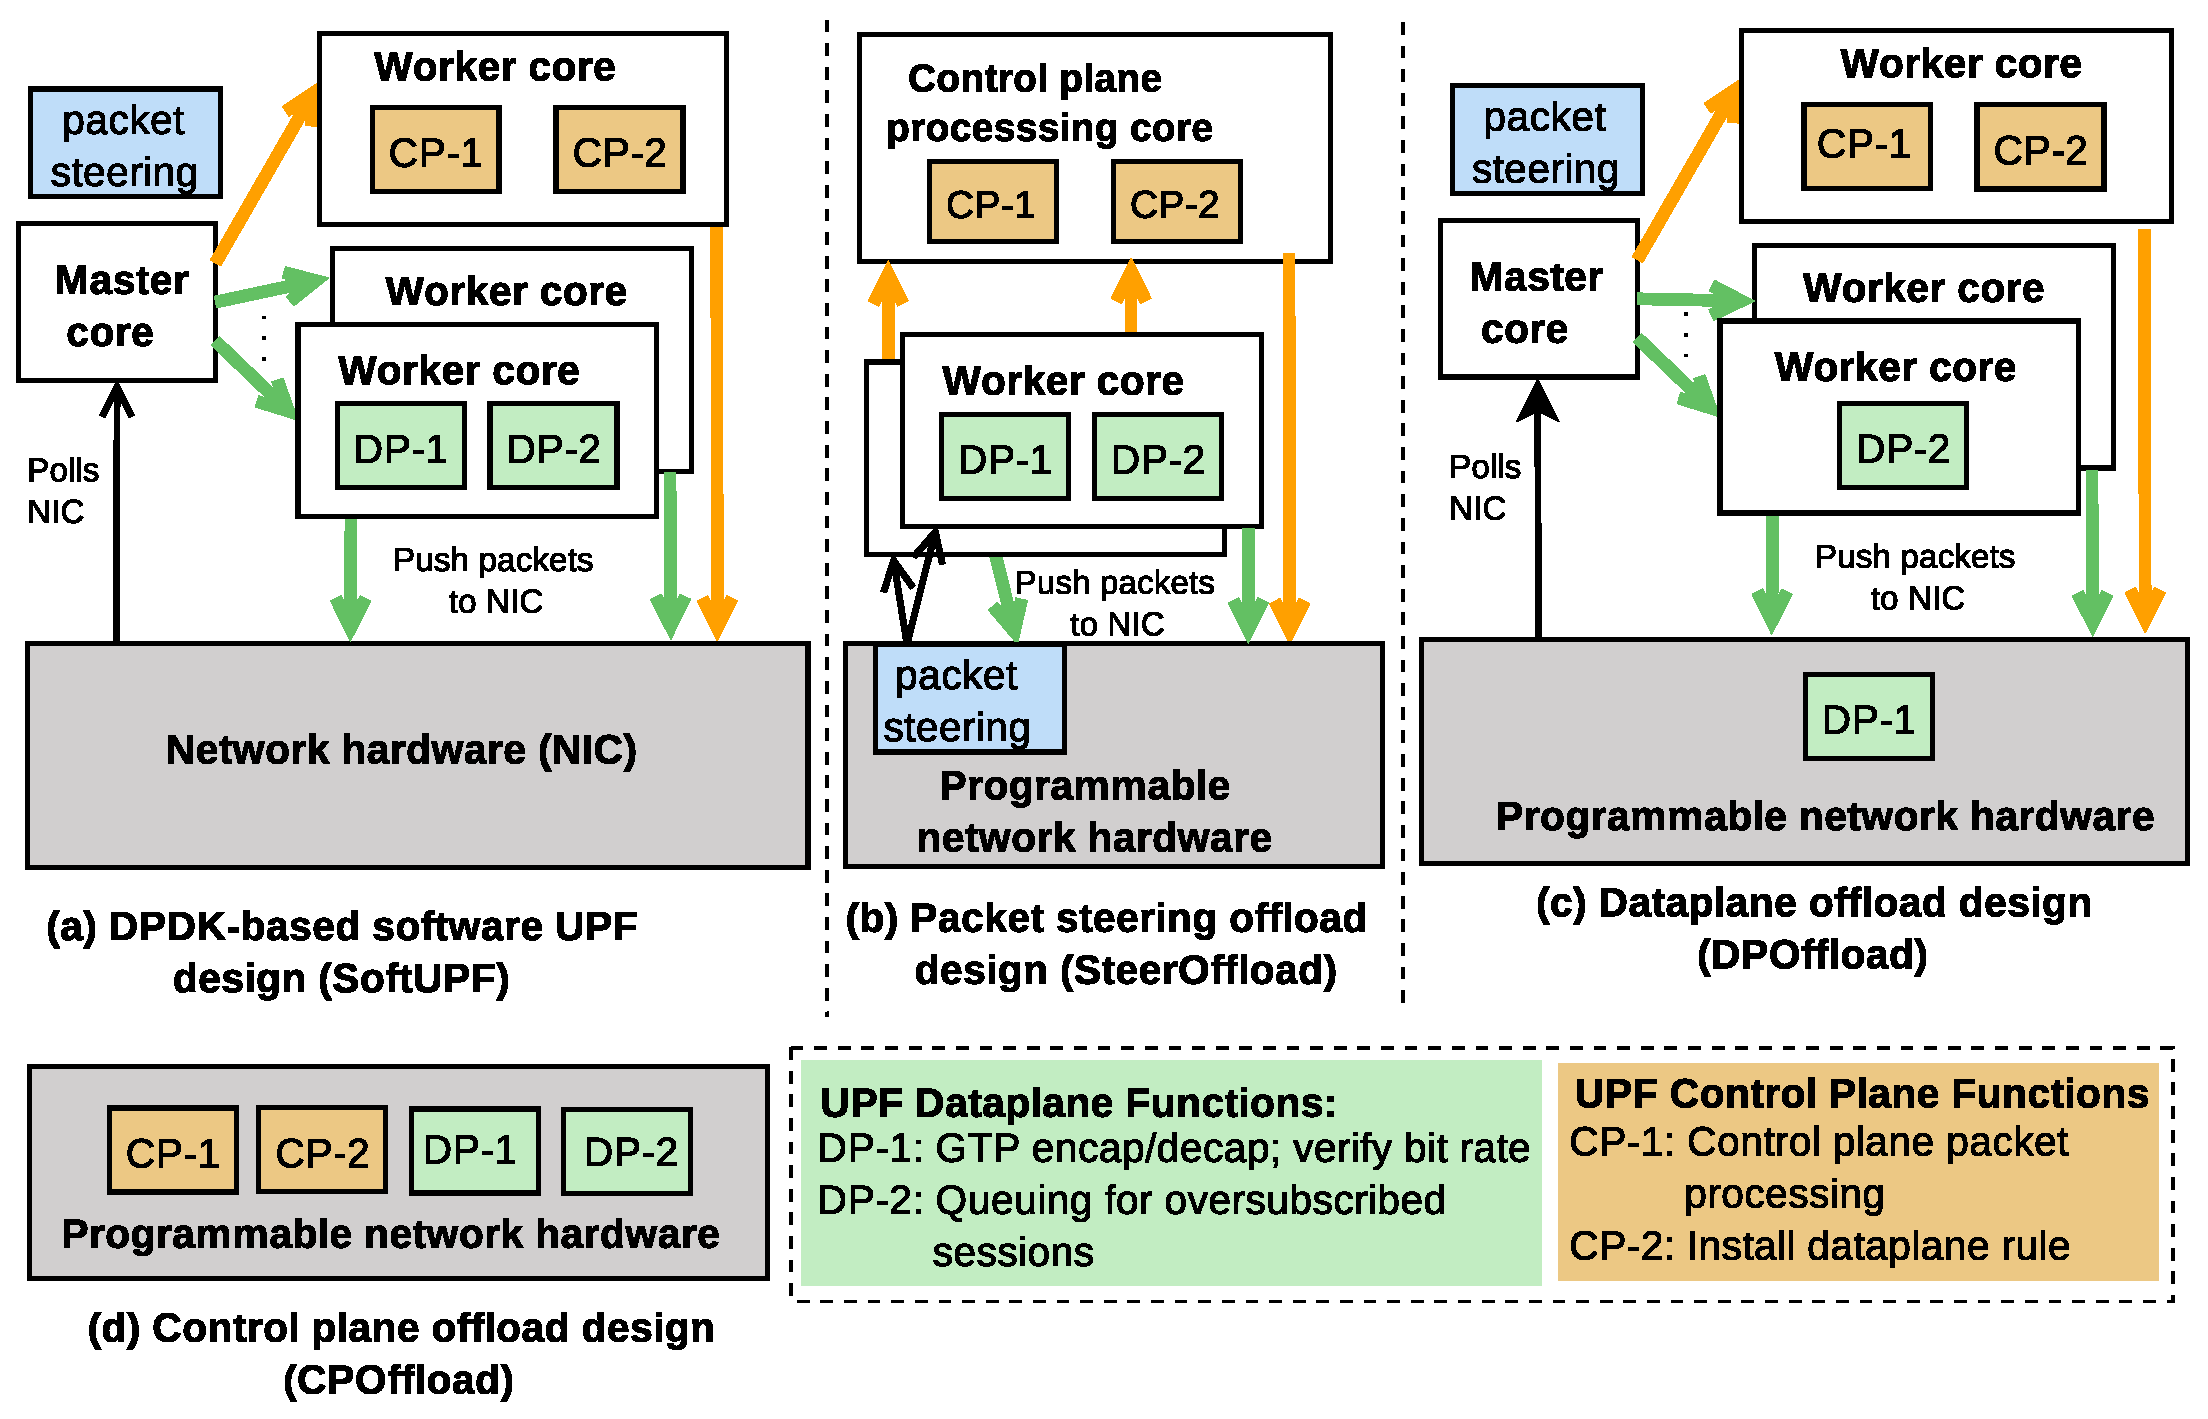
\includegraphics[width=0.48\textwidth]{fig/all_designs.eps}
 \setlength{\abovecaptionskip}{-5pt}
\setlength{\belowcaptionskip}{-12pt}
 \caption{5G User Plane Function designs.}
 \label{fig:all_designs}
\end{figure}
% \vspace{-2pt}
This section describes the various UPF prototypes compared in this paper, beginning with a software-based UPF, and progressively moving towards UPFs that offload more functionality to programmable hardware, as shown in Figure~\ref{fig:all_designs}.

% XXX: Figure needs changes. Talk to me (Mythili) for comments.
% Design overview with a picture that shows the 5G components with their placement in each design
% what is our design/implementation? what are challenges? what were the possible choices? what/why did we choose XYZ? 
\vspace{-3mm}
\subsection{DPDK-based software UPF} 
\label{sub:swUPF}

We begin with describing our purely software DPDK-based UPF (Figure~\ref{fig:all_designs}a) that is representative of the most common UPF design used in production networks today. Our implementation is based on a fully standards-compliant UPF obtained from~\cite{5g-testbed, 5g-testbed-in}. Our UPF supports GTP-based forwarding and AMBR-based QoS enforcement (using a variant of the algorithm in~\cite{carousel}), among other features. Our implementation spans $6.5K$ lines of code. Our UPF has a pipeline-based design, with multiple master and worker threads, each pinned to separate CPU cores. The master threads receive packets from the NIC via the polling-based DPDK APIs, and distribute them to the worker threads for further processing. PFCP packets and dataplane packets are processed by separate worker cores. The inter-core communication between the master and workers is done via the lockless shared rings provided by DPDK, for efficiency and high performance. The worker threads continuously poll the shared rings for received packets, process them, and transmit the output.

When steering packets to worker cores, we would like to ensure that the traffic of a UE is processed by the same worker, in order to avoid splitting the state of a particular UE (forwarding rules, buffered packets, and so on) across multiple workers. This steering is achieved by using the hash over the TCP/IP headers of the``inner'' IP datagram (the datagram originated by the UE, which has been encapsulated within GTP for transit through the core) to partition traffic to worker cores. Note that we cannot simply use a hash over the ``outer'' UDP/IP header fields because dataplane traffic of all UEs between a gNB-UPF pair arrives on the same UDP link, so the outer IP header fields cannot be used to differentiate UEs.  Most modern NICs have the capability to distribute packets to multiple CPU cores via RSS~\cite{rss}; however, the set of header fields used for RSS is restricted to the outer IP header fields. Therefore, a purely software-based DPDK design cannot rely on the NIC to perform packet steering based on the inner IP header fields, and must perform this steering in software.  (RSS based on outer header fields is still useful to distribute traffic to multiple master cores for performance scaling.) Packet steering in software also allows the UPF to efficiently rebalance load across worker cores in case some worker cores are more overloaded than others, and to dynamically scale to more worker cores quickly on demand. In our design, the master cores periodically monitor the queue lengths of the lockless rings shared with the worker cores, and reassigns UEs across workers if it finds that a worker core is overloaded (as inferred from a persistently high queue length), and another underloaded. If all worker cores are overloaded, the master can spawn a worker on new CPU core (when available). We have only implemented a simple load balancing algorithm, but more complex algorithms that assign special classes of UEs (e.g., high priority UEs) to specific worker cores are also possible. 

%While it is recomended that NICs perform RSS over the inner IP fields to distribute packets to worker cores, having capability to perform RSS w.r.t inner IP fields are recommended for distributing packets uniformly across different master cores, but not mandatory in this design. Considering a real-world scenario with multiple RANs so that outer IP fields will have different source addresses, even if the NIC non-uniformly distribute the data packets across master cores based on some RSS hashing, the master cores themselves will re-distribute the packets to worker cores uniformly in the s/w. Thus, this design provides us an option to scale up even with simple NICs.\\

%\noindent \textbf{Implementation details:}
%\begin{itemize}
%    \item The implementation spans $~XX$ lines of code.
%    \item For our 2-NIC setup, we need at least 2 master cores, one polling for packets coming from the RAN and another polling for packets coimg from the DNN. We cannot use only 1 master core it will degrade the performance.
%    \item Although in pipeline design we can process both UL and DL packets in the same worker cores, they are processed in separate worker cores. This decopuling is done to improve performance.
%\end{itemize}
%\noindent \textbf{Advantages:} Doing everything in s/w provides more flexibility in terms of packet distribution or QoS enforcement not available in other designs where some of the computation is offloaded to the h/w.
%\begin{itemize}
%    %\item Since packet distribution happens in s/w, we can use any advanced heuristic instead of simply hashing. For example, we can dedicate all packets from a heavy-hitter UE to only a particular set of worker cores. In future implementations, we can also use heuristics like predicting the load on worker cores beforehand and distributing accordingly.
%    \item Since packet distribution happens in s/w, if a worker core (say, core A) is saturated by some heavy-hitter UEs, we can dynamically balance the load by redirecting packets to other unsaturated worker cores instead of sending them to core A.
%    \item Assuming there are enough master cores, scaling up/down of worker cores is easy and seamless.
%\end{itemize}
%\noindent \textbf{Limitations:}
%\begin{itemize}
%    \item Inter-core communication as well as performing everything in the s/w incurs a computational overhead. As a result, the performance is expected to be less and the latency is expected to be higher than other prototypes which offload some of the computation to the h/w.
%\end{itemize}


\vspace{-8pt}
\subsection{Packet steering offload}
\label{sub:steerOffload}

In our next design (Figure~\ref{fig:all_designs}b), the steering of UE traffic to cores happens not in software but within the NIC itself. This design relies on advanced NICs that allow RSS based on inner IP headers. For example, Intel NICs support the Dynamic Device Personalization~\cite{ddpGuide} feature on 40Gbps+ NICs,  which enables parsing of the GTP header and inner TCP/IP header fields for hash computation. Because the input to the hash function now contains the UE's IP address and GTP tunnel identifier, the packets of a UE are redirected to the same receive queue and CPU core via RSS. The multiple worker threads of the DPDK-based software UPF are assigned dedicated hardware receive queues and directly receive traffic from their corresponding queues. The worker threads then process the received packets in a run-to-completion model. The control plane traffic is redirected to (and processed on) dedicated cores as before. This design represents the simplest possible offload that can be done to programmable hardware, and is used by state-of-the-art UPFs~\cite{astri, intel_wp, mavenir, metaswitch}. 

Offloading packet steering to hardware provides higher throughput and lower latency, due to minimal inter-core communication in software and faster hash computation in hardware. However, this design is also less flexible as we have lesser control on assigning UEs to cores. For example, the DPDK i40e poll mode driver~\cite{i40eDriver} does not support dynamic load balancing by remapping queues to cores based on load. Further, dynamic scaling is also complicated by the fact that one needs to stop and reconfigure the port in order to change the number of receive queues.

%The advantages that the RTC offers above the pipeline design is higher throughput and lower latency. The higher throughput and lower latency is due to minimal inter-core communication and faster hash computation in the hardware.
%%
%The major limitation is the rigidity and inflexibilty. It is not possible to steer
%flows from one heavily loaded core to a relatively idle core as the only way to
%redirect flows is hash computation in hardware. Pipeline offers this flexibility
%as redirection is in software. DPDK i40e poll mode driver does not offer dynamic load balancing \cite{i40eDriver} by remapping queues to the cores based on the load characteristics of  different cores.
%It is also not possible to scale the number of worker cores with the increasing load without stopping and reconfiguring the port.

%The packets in the uplink direction from RAN to the DNN (the Internet) are GTP encapsulated packets \cite{5g29060} The hash of the GTP header and the inner IP is computed in hardware and the packets are directed to the corresponding queue. Each core draws packets from a specific mapped queue.
%Receive side scaling (RSS) is used for the packet redirection.
%A standard RSS hash computation occurs on the outer packet fields . These fields are
%identical for a given RAN-UPF pair and the packet redirection is not successful with the standard RSS.
%Packet redirection in the hardware requires parsing of inner packet fields for getting the required entropy in hash computation. Intel has provided dynamic device personalization \cite{ddpGuide}
%feature on 40Gbps+ NICs which enables parsing of GTP header and inner
%packet fields for hash computation.
%This input contains tunnel endpoint ID, inner UE IP etc. which is unique for a given flow.
%Each flow is mapped independently and stays pinned to a specific core.
%
%The packets in the downlink direction are not encapsulated and have sufficient entropy in the headers for uniform distribution among the cores.
%
%
%Each data plane core after receiving the packet processes it completely and independently of other cores before forwarding it further.
%The control plane packets and other packets which are not in data plane are sent to
%the first registered queue due to failed parsing. Sending these packets to the control plane core
% is the only inter-core communication overhead.
%
%
%The advantages that the RTC offers above the pipeline design is higher throughput and lower latency. The higher throughput and lower latency is due to minimal inter-core communication and faster hash computation in the hardware.
%
%The major limitation is the rigidity and inflexibilty. It is not possible to steer
%flows from one heavily loaded core to a relatively idle core as the only way to
%redirect flows is hash computation in hardware. Pipeline offers this flexibility
%as redirection is in software. DPDK i40e poll mode driver does not offer dynamic load balancing \cite{i40eDriver} by remapping queues to the cores based on the load characteristics of  different cores.
%It is also not possible to scale the number of worker cores with the increasing load without stopping and reconfiguring the port.
%Prateek

\input{desCD}

% \vspace{-3mm}
\vspace{-8pt}
\subsection{Control plane offload} 
\label{cp-offload}
% Key points to expand:
% \begin{itemize}
%  \item Need (end of prev design/start of this design): Offload of dataplane functions to the hardware not enough. Control plane processing in software results in high latencies for initiating data traffic. Also, control plane traffic is increasing exponentially with the 5G applications
% We have a design to implement variable header depth/layers using recirculation strategy but have not implemented in the current evaluation.
%  \item Procedures involved in control plane processing: (1) Parsing PFCP packet with recursive headers that carry session/flow related information such as the session identifier, QoS information for the flow, tunnel identifers for GTP tunneling. (2) Installing rules to the data plane hardware for data plane processing offload.
%  \item Challenges: (1) PFCP packet parsing: Variable parse tree depth (2) Memory to store state for millions of users (3) Install and update the forwarding rules within the data plane at line-rate
%  \item Solution choices? What we choose? What is yet to be addressed?
% \end{itemize}

In the dataplane offload design (Figure~\ref{fig:all_designs}c), signaling messages that configure the dataplane are still handled in userspace. As a result, a workload with a large number of signaling messages may slow down the hardware dataplane, due to a bottleneck at the software that configures hardware rules. To overcome this limitation, we implement a UPF design which offloads signaling message processing also to programmable hardware (Figure~\ref{fig:all_designs}d). %Our control plane offload implementation spans 500 lines of P4 code that run on our Agilio CX 2x10GbE smartNIC~\cite{netronome}. 
In this design, we move away from storing forwarding/QoS rules of a session in match-action tables (which need to be updated via the controller running in userspace), and store them instead in P4 register arrays. The register data structure supports update operations to register array state within the dataplane pipeline at linerate, but cannot perform key-based lookup. When a control plane PFCP message for a particular session arrives, we map the 64-bit session identifier to a 24-bit index into the register array. We can then access or manipulate the corresponding session state directly from within the dataplane, without requiring the intervention of the userspace controller. Since our index calculation is (currently) not collision-free, we store additional state in the register array to validate if we are accessing the correct session. In case of a collision or session mismatch, the control plane message is forwarded to the userspace for processing. We also make a few simplifying assumptions when parsing PFCP messages in our current implementation. For example, we assume a PFCP header with fixed structure that fits within the hardware memory, whereas in practice, the PFCP header comprises of a variable length component that consists of recursive PDR, FAR, and QER (\S\ref{sec:bg}) headers.  We defer the comprehensive handling of complex PFCP messages to future work.

%Note that the control plane processing in software with or without offload is substantial ($\sim$ XXX ms), which results in high latencies for data traffic initiation. A 5G traffic characterization study~\cite{5g-iot-chk} for IoT applications shows that certain use-cases such as massive broadband and critical IoT generate large amount of control plane traffic per user (or device) and require strict latency SLAs. The 5G specification requirement is to support connection density up to 150K connections $/km^2$ which adds to the increased control plane processing demand. 

%We can store the session forwarding/QoS state on the programmable hardware's {\em table} data structure for stateful packet processing.
%Control plane processing requires updates to the session state. The table data structure updates in hardware are performed by the control plane that runs in user-space (slow path processing), resulting in higher control plane processing latency. 
%
%The {\em register-array} data structure supports update operations to register-array state within the data plane pipeline at line-rate, but cannot perform key-based lookup. 
%We design a simple hash function to index into the register-array data structure to access or manipulate the corresponding session state within the data plane. Since the hash function is not collision-free, we store additional state in the register array to validate if we are accessing the correct session. In case of a collision, the control plane message is forwarded to the user-space for processing. 

%As discussed in~\S\ref{sub:5g_arch}, the UPF control plane is responsible for processing session establishment, session modification, and session deletion request procedures. The processing of these control plane procedures involves
%(1) parsing PFCP messages received from SMF which carry session related information such as the session identifier, user IP address, QoS information for the flow, tunnel identifers for GTP tunneling, (2) generation of PFCP response messages, (3) store user's session state, and (4) install rules over the programmable hardware to support data plane forwarding and QoS enforcement for any given session. We encounter the following challenges with the UPF control plane offload design.
% 
% \noindent {\textbf{Challenges.}}

%\noindent {\textbf{PFCP header parsing.}} 
%The PFCP header comprise of a variable length component that consists of recursive PDR, FAR, and QER (\S\ref{sub:5g_arch}) headers. The parsing of such packets would require deep packet processing pipelines, which may not be supported by the programmable hardware. The PFCP header size could be large and may not fit into the memory reserved for packet headers within the programmable hardware.
%
%We assume PFCP header with fixed structure that fits within the hardware memory. 
%
%\noindent {\textbf{Slow state updates.}}

%\noindent {\textbf{Limited memory to store UE's session state.}}
%We need to store the state for 10s of millions of sessions, but the programmable hardware has limited memory (19MB for Netronome CX-4000 smartNIC~\cite{netronome}). 
%
%There is a limit on the number of user sessions supported on one programmable hardware switch, but we can further scale using multiple hardware switches or use hardware that has more on-board memory.
%
%\noindent {\textbf{Implementation.}}
%Our current implementation uses Agilio CX 10bE smartNIC~\cite{netronome} for UPF control plane processing offload. The packet processing pipeline for control plane procedures is implemented using P4 language. The hash function uses the 64-bit session identifier as input and provides a 24-bit value. This function simply selects the subset of the session identifier bits. 
%The session state stored in the register arrays includes the session identifier, UE's IP address, the uplink/downlink tunnel identifiers for GTP processing. We also populate the register array structure with forwarding and QoS state that can be used for data plane GTP-based forwarding. Our current implementation can store the UPF control plane processing state for {\em 16M} users and spanned around {\em 500}  lines of code.


%\subsection{Other 5G Network Functions and emulators for load generation }
{\textbf{XXX: Can go in the eval section?}}
\noindent \textbf{RAN design:} 
We use a multi-core DPDK application which acts as a RAN emulator. Normally, it acts as a standard complaint NF. However, during UPF load testing, the RAN acts as an open-loop load generator and other NFs are bypassed to avoid any bottlenecks and saturate the network bandwidth. For instance, during Control Plane load testing, SMF is not involved and RAN itself crafts and sends standard complaint PFCP packets to the UPF. Similary, in the Data Plane, the RAN creates multiple GTP packets beforehand (with different GTP TEID and different inner IP source addresses) to simulate load from multiple UEs and sends them to the UPF in a round robin fashion once the test starts.\\
Our RAN implementation spans $~XX$ lines of code.

\noindent \textbf{DNN design:}
Our DNN is also a multi-core DPDK application which acts as a sink, mirror, or load generator depending on our experiments. For example, when we want to simulate only DL traffic, the DNN acts as an open-loop load generator capable of saturating the network bandwidth. Similar to our RAN, the DNN also manually crafts IP packets beforehand. The IP destination addresses are made different to simulate multiple UEs.\\
Our DNN implementation spans $~XX$ lines of code.

\noindent \textbf{AMF/SMF:}
Not involved in CP/DP load test. Part of testbed. Should we include desc of these?

\vspace{-5pt}
\section{Evaluation} \label{sec:eval}

% \begin{itemize}
%  \item Draw the testbed figure. 
%         Intel Xeon processor (2.2 Ghz, 24 cores)
%         128 GB RAM
%         10G NIC connected via cable (P2P)
%         DPDK installed in Server 2 (v 19.11). 2MB hugepages used.
%         A \& B:	40G NIC, Intel XL710 i40e (QSFP+ cables)
%         C,D,E:     10G Netronome nfp 
%         RAN machine: RAN emulator. DPDK load generator. Same processor as UPF
%         DNN machine: DPDK sink/mirror/load generator. Same processor as UPF
%      
%  \item Describe the testbed for design A/B, design C/D/E. This includes the server configurations (CPU+memory) and connection info, the NIC info (model, bandwidth), DPDK version info, python controller. 
%  \begin{itemize}
%   \item Add the common configuration/setup for all designs first
%   \item Add specific configuration/setup: design A+B, design C+D, design E
%  \end{itemize}
% 
%  \item Parameters and metrics: Describe how our load is generated? What is the duration of our experiments? Describe the traffic distribution used/varied (imix, UL/DL ratios) in a table, and highlight the standard workloads (imix, 1:2 UL:DL) along with appropriate citation. Explain the metrics evaluated (throughput, latency, compute cost, power dissipation).
%  \item Add placeholders for graphs and experiment details in individual subsections (AvsB etc).
% \end{itemize}

We now evaluate our various UPF designs and quantify the performance gains of offloading UPF functionality.

% \begin{figure}[ht]
%  \centering
% \includegraphics[width=0.3\textwidth]{fig/5g_testbed.png}
%  \setlength{\abovecaptionskip}{6pt}
% % \setlength{\belowcaptionskip}{-6pt}
%  \caption{Testbed setup for 5G User Plane Function.}
%  \label{fig:testbed}
% \end{figure}
\noindent \textbf{Experiment Setup.} All our experiments run on three servers with Intel Xeon processors (2.2Ghz, 24 cores) and 128GB RAM. The first server runs a RAN emulator/load generator that generates emulated traffic to the UPF, comprising of control plane PFCP messages and uplink/downlink dataplane traffic from a large number of UEs. The RAN emulator runs over DPDK to generate traffic at a high rate and we ensure that it can generate enough load to saturate the control/data plane of the UPF in all experiments. The second server in our setup runs one of the versions of our UPF. The third server runs a sink application that generates downlink traffic and consumes uplink traffic from the RAN emulator. Our RAN emulator and sink span 12K lines of code. We use two sets of NICs in our experiments. For experiments which evaluate the impact of offloading packet steering, we connect the servers using Intel XL710 i40e 40Gbps NICs that are capable of offloading packet steering. For the rest of the experiments, we use Agilio CX 2x10GbE programmable NICs~\cite{netronome}. 

%Our software UPF code runs on DPDK v19.11 and uses 2MB hugepages. 
\noindent {\textbf{Parameters and metrics.}} 
% We generate different traffic mixes for dataplane experiments by varying the packet size, uplink/downlink traffic ratio, and the percentage of ``oversubscribed'' sessions where the incoming load exceeds the QoS-prescribed rate limit, as shown in Table~\ref{tab:workload-scenarios}. These scenarios also include a typical traffic mix found in real user traffic~\cite{imixLink, 4g-uldl, 5g-uldl}. 
We generate different traffic mixes for dataplane experiments by varying the packet sizes, across $64B$, $1400B$ and a typical traffic mix~(``IMIX'') found in real user traffic~\cite{imixLink}. We use an uplink to downlink traffic ratio of 1:2~\cite{4g-uldl, 5g-uldl}. 
% and the uplink to downlink traffic ratio as $1:2$~\cite{4g-uldl, 5g-uldl}.
% (XXX: Are we including oversubscribed flows?)
Control plane traffic consists of sets of session creation, modification, and deletion PFCP messages processed one after the other---we refer to this set as a control plane ``procedure''. All results reported are for an experiment conducted for 300 seconds, unless mentioned otherwise. We show error-bars that denote the maximum and minimum values where applicable. The performance metrics measured are the dataplane throughput (bps or pps), control plane throughput (procedures/sec), and average end-to-end response latency (RTT, where the response is mirrored by sink for data packets, and is generated by the control plane processing for signaling packets), as measured at UPF saturation. For experiments evaluating the effect of offloading packet steering, we send data from $65K$ concurrent users. For experiments involving dataplane and control plane offload to smartNICs, we emulate $1K$ concurrent users.

%\begin{table}[t]
%\begin{scriptsize}
%\begin{center}
%\def\arraystretch{1.5}%  1 is the default, change whatever you need
%\begin{tabular}{|p{1cm}|p{1.5cm}|p{1.9cm}|p{2.3cm}|}\hline 
%{\bf{Scenario}} & {\bf{Packet size}} & {\bf{Uplink:Downlink}} & {\bf{Oversubscribed flows\%}} \\ \hline 
%{\bf{Typical}} & imix~\cite{imixLink}  & 1:2~\cite{4g-uldl, 5g-uldl} & 1 \\ \hline
%{\bf{T\_1}} &  imix & 1:2 & 25 \\ \hline
%{\bf{T\_2}} & imix  & 1:2 & 0 \\ \hline
%{\bf{T\_3}} & 64B  & 1:2 & 0 \\ \hline
%{\bf{T\_4}} & 1400B  & 1:1 & 0 \\ \hline
%{\bf{T\_XXX}} &   &  &  \\ \hline
%\end{tabular}
%\setlength{\abovecaptionskip}{-6pt}
%% \setlength{\belowcaptionskip}{-10pt}
%\caption{Dataplane workload scenarios.} 
%\label{tab:workload-scenarios}
%\end{center}
%\end{scriptsize}
%\end{table}

% XXX: Please give suitable names for the various designs in the legends and captions. 



% Experimental setup
% Load generation parameters and metrics evaluated

% \subsection{Packet Steering Offload}
\noindent  {\textbf{Packet Steering Offload.}} We begin by evaluating the impact of packet steering to programmable NICs, and compare a pure software-based UPF (\S\ref{sub:swUPF}) with a UPF that offloads packet steering to programmable hardware (\S\ref{sub:steerOffload}). Figure~\ref{fig:AvsB_tput} shows the throughput and latency of both the designs when we dedicate $2$ cores for dataplane processing---one for uplink traffic and another for downlink traffic. As expected, we find that offloading packet steering leads to $45 \%$ higher throughput and up to $37 \%$ lower latency (except when both designs saturate linerate at maximum packet size), due to lesser overhead of intercore communication and packet steering in the offloaded design. However, the performance gains due to this offload also come with a loss in flexibility. We consider a scenario where a UPF has to dynamically scale the number of cores it is running on due to an increase in incoming traffic. Figure~\ref{fig:AvsB_dyn_scl} shows the UPF throughput during scaleup, and we see the adverse impact of having to restart the port and reconfigure hardware queues in the offload design. Next, we configure our RAN emulator in such a way that 20\% of the UEs processed by a single worker core generate a sudden burst of traffic, and Figure~\ref{fig:AvsB_rebal} shows how the offload design suffers high latency due to its inability to balance load across cores in the presence of such ``heavy-hitter'' UEs. {\em In summary, we find that offloading packet steering to NICs leads to significant performance gains, but comes at a loss of flexibility that can hurt operators that expect to perform dynamic scaling frequently or see skewed traffic across users. }
%Note that both the designs are scalable across cores. SoftUPF takes $3$ and $4$ cores to saturate $40G$ linerate in the uplink and downlink respectively. In contrast, the SteerOffload design takes $2$ and $3$ cores to saturate uplink and downlink respectively. 
%deally, the latency after rebalancing should be same as when there was less load. But we observe that there is a slight increase in the heavy hitter latency. We have also noticed that this latency after rebalancing further increases if the load from heavy hitter UEs is increased further. This is because we have used a very simple rebalancing algorithm which is sub-optimal. We expect that an optimal algorithm with a better heuristic will prevent/reduce this increase in latency, and consider it as one of our future works. However, even with this sub-optimal algorithm and increase in latency, we see that this is still less than the RTT latency for a heavy hitter in the RTC design.
% \begin{figure}[t]
% \centering
%   \begin{tabular}{@{}cc@{}}
%     \includegraphics[width=.25\textwidth]{graphs/dynScaling_softUPF} &
%     \includegraphics[width=.25\textwidth]{graphs/dynScaling_SteerOffload}    \\
%   \end{tabular}
%    \caption{SoftUPF vs SteerOffload: Dynamic Scaling.}
%  \label{fig:AvsB_dyn_scl}
% \end{figure}

% \begin{figure}[t]
%  \centering
% \includegraphics[width=0.45\textwidth]{graphs/pipelineVsRTT}
%  \setlength{\abovecaptionskip}{4pt}
%  \setlength{\belowcaptionskip}{-12pt}
%  \caption{SoftUPF vs. SteerOffload: Performance.}
%  \label{fig:AvsB_tput}
% \end{figure}
% 
% \begin{figure}[t]
%     \centering
%      \includegraphics[width=0.4\textwidth]{graphs/dynScaling} % second figure itself
%      \setlength{\abovecaptionskip}{4pt}
%      \setlength{\belowcaptionskip}{-8pt}
%  \caption{SoftUPF vs. SteerOffload: Dynamic Scaling.}
% %  \caption{Dynamic Scaling.}
%  \label{fig:AvsB_dyn_scl}
% \end{figure}
% 
% % \begin{figure}[t]
% %     \centering
% %     \begin{minipage}{0.235\textwidth}
% %         \centering
% %         \subfloat[SoftUPF]{\includegraphics[width=\textwidth]{graphs/dynScaling_softUPF}} % first figure itself
% %     \end{minipage}
% % \hfill
% %     \begin{minipage}{0.235\textwidth}
% %         \centering
% %          \subfloat[SteerOffload]{\includegraphics[width=0.99\textwidth]{graphs/dynScaling_SteerOffload}} % second figure itself
% %     \end{minipage}
% %      \setlength{\abovecaptionskip}{4pt}
% %      \setlength{\belowcaptionskip}{-12pt}
% %  \caption{SoftUPF vs SteerOffload: Dynamic Scaling.}
% %  \label{fig:AvsB_dyn_scl}
% % \end{figure}
% 
% \begin{figure}[t]
%  \centering
% \includegraphics[width=0.4\textwidth]{graphs/heavyHitter}
%  \setlength{\abovecaptionskip}{4pt}
%  \setlength{\belowcaptionskip}{-8pt}
%   \caption{SoftUPF vs. SteerOffload: Heavy hitters.}
% %  \caption{SoftUPF vs SteerOffload: Heavy hitter redistribution.}
%  \label{fig:AvsB_rebal}
% \end{figure}

% XXX: can combine throughput and latency in one graph with two y-axis, when showing results for different scenarios.

% XXX: Are throughput results for single core?

% XXX: need a graph to show throughput as a function of number of cores. This is only place where we show DPDK UPF hitting linerate. Or at least mention in the text that performance scales with cores and we can saturate linerate at XXX cores.  

% XXX: Keep the dynamic scaling and heavy hitter graphs simple, with one load change/scaling event. Do not clutter with datapoints.


\input{AvsCD}

% \subsection{Control Plane Offload}
\noindent  {\textbf{Control Plane Offload.}} Next, we compare the control plane performance of three designs: the pure software UPF (\S\ref{sub:swUPF}), the design that offloads only the dataplane forwarding to programmable hardware but processes control plane packets in userspace (\S\ref{sub:dpOffload}), and our preliminary implementation of a UPF that offloads even control plane processing to programmable hardware (\S\ref{cp-offload}). Table~\ref{tab:perf-cp-offload} shows the average rate of processing signaling messages, and the processing latency, for all three designs. We observe that only offloading dataplane processing to hardware has a significant adverse impact on control plane performance, because the performance is limited by the overheads of control plane message processing in software and the subsequent communication with NIC firmware. Therefore, the design that offloads only dataplane processing has 86\% lower control plane throughput and 15$\times$ higher control plane latency, as compared to the pure software UPF. However, the UPF that offloads control plane processing has 402$\times$ higher throughput  as compared to the pure software design, and $3K\times$ higher throughput as compared to the dataplane offload design. It also has 77\% latency reduction compared to the pure software design, and  98\% latency reduction compared to the dataplane offload design. This result points to the conclusion that offloading GTP-based dataplane processing alone to programmable hardware is likely to cause additional performance concerns for signaling message processing, especially for future 5G networks that expect to have frequent signaling with IoT devices. {\em A comprehensive programmable dataplane accelerated UPF must offload signaling message processing to hardware as well, in addition to offloading dataplane processing.}

% $18636\times$ 

% \begin{table}[t]
% \begin{scriptsize}
% \begin{center}
% \def\arraystretch{1.5}%  1 is the default, change whatever you need
% \begin{tabular}{|p{2.4cm}|p{1.1cm}|p{2cm}|p{1.2cm}|}\hline 
% % {\bf{Performance metric}} & {\bf{DPDK-based software UPF}} & {\bf{Dataplane offload}} & {\bf{Control plane offload}} \\ \hline 
% {\bf{Performance metric}} & {\bf{SoftUPF}} & {\bf{DPOffload}} & {\bf{CPOffload}} \\ \hline 
% {\bf{Throughput}} & 5.1K  & 666  & 2.05M  \\ \hline
% {\bf{Latency}} & 113$\mu s$  & 893 $\mu$s & 26$\mu s$ \\ \hline
% % {\bf{Performance per USD}} & 88  & 1 & 4.6K  \\ \hline
% % {\bf{Performance per Watt}} & 40  & 1 & 41K \\ \hline
% \end{tabular}
% \setlength{\abovecaptionskip}{-8pt}
% \setlength{\belowcaptionskip}{8pt}
% \caption{Control plane performance.} 
% \vspace{-4mm}
% \label{tab:perf-cp-offload}
% \end{center}
% \end{scriptsize}
% \end{table}


\vspace{-5pt}
\section{Conclusion and Future Work} \label{sec:future}

% Abhik : ==== Start
% 1. Control plane mediated oversubscribed flow detection and send oversubscribed flow back to dataplane if they remains undersubscribed for a certain time.
% 2. Some possible extension of plan D
% Abhik : ==== End

Our work evaluates several designs of the 5G user plane function (UPF) that leverage programmable dataplane hardware in different ways to improve performance. Our evaluation highlights the costs and benefits of each offload strategy, and provides lessons for future research in this area. We find that UPF offload designs proposed in prior work improve performance, but hurt flexibility in dynamic workload scenarios, and cannot process signaling traffic efficiently. To fully realize the power of programmable hardware offload for UPFs, we need to overcome the technical challenge of being able to parse complex 5G signaling messages in hardware. Our work is a first step towards using programmable dataplanes to realize the vision of 5G. 
% Discuss the promising ideas for the future 5G UPF (or more) design.

\vspace{-5pt}
\section*{Acknowledgements}
We thank the 5G testbed project, funded by the Department of Telecommunications, Govt. of India, for access to 5G UPF.

\vspace{-9mm}

% Abhik: Add or remove ~\\ (blank newline) here to overcome href out of boundery error
%~\\
% \bibliographystyle{ACM-Reference-Format}
\bibliographystyle{plainnat}
\interlinepenalty=10000
\bibliography{reference}

% Paper structure
% 1. Intro
% 
% 2. Background & related work
% 
% 2.1 Basics of 4G/5G, industry, academia: Pure DPDK, steering packet forwarding : Diptyaroop
% 
% 2.2 Programmable data planes:  5G offload + general in-network compute
% 
% 3. Design & implementation
% A:Diptyaroop, B:Prateek, C+D:Abhik, E:Rinku
% 
% 4. Evaluation
% Avs.B:Diptyaroop+Prateek, Avs.C+ Avs.D:Abhik, Avs.E+Cost/power:Rinku 
% 
% 5. Discussion/Conclusion
% Only GTP offload is not enough + signalling 
%

\end{document}

%Reference changes: [25] P4: programming ... -> SIGCOMM full form?
% [27] APnet full form (
% [28] Meter: Title change to P4 meter
% [40] In band nw telemetry (SIGCOMM full form)
% Hotnets full form
% All SIGCOMM, APNet, Hotnets
% switchml --> how to show arxiv
